% Generated by my modifications to the default Pandoc beamer template.
% Karl Browman has a tutorial about how to make Beamer sane:
% http://kbroman.wordpress.com/2013/10/07/better-looking-latexbeamer-slides/

% 12pt by default; handout if the handout template variable is defined
%\documentclass[12pt,ignorenonframetext,handout,12pt]{beamer}
\documentclass[12pt,handout]{beamer}
\usetheme{metropolis}

\providecommand{\tightlist}{%
  \setlength{\itemsep}{0pt}\setlength{\parskip}{0pt}}


% theme, colortheme, and fonttheme with sensible defaults
%%\usetheme{metropolis}
%%%\usecolortheme{dove}
%%
% if it is a handout show the notes text; otherwise don't
\setbeameroption{hide notes}
\setbeamertemplate{note page}[plain]

% Don't show things we don't want to see
\beamertemplatenavigationsymbolsempty
\hypersetup{pdfpagemode=UseNone} % don't show bookmarks on initial view

% Slide number in lower right
\definecolor{gray}{RGB}{155,155,155}
\setbeamertemplate{footline}{%
    \raisebox{5pt}{\makebox[\paperwidth]{\hfill\makebox[20pt]{\color{gray}
          \scriptsize\insertframenumber}}}\hspace*{5pt}}

% Space between paragraphs on notes page
\addtobeamertemplate{note page}{\setlength{\parskip}{12pt}}

% Color and shape of bullets
% \setbeamercolor{item}{fg=gray} 
% \setbeamercolor{subitem}{fg=gray}
% \setbeamercolor{itemize/enumerate subbody}{fg=gray}
\setbeamertemplate{itemize item}{{\textendash}}
\setbeamertemplate{itemize subitem}{{\textendash}}
\setbeamerfont{itemize/enumerate subbody}{size=\footnotesize}
\setbeamerfont{itemize/enumerate subitem}{size=\footnotesize}

\usepackage{amssymb,amsmath}
\usepackage{ifxetex,ifluatex}
\usepackage{fixltx2e} % provides \textsubscript
\ifxetex
  \usepackage{fontspec,xltxtra,xunicode}
  \defaultfontfeatures{Mapping=tex-text,Scale=MatchLowercase}
\else
  \ifluatex
    \usepackage{fontspec}
    \defaultfontfeatures{Mapping=tex-text,Scale=MatchLowercase}
  \else
    \usepackage[utf8]{inputenc}
  \fi
\fi
\usepackage{longtable}
% These lines are needed to make table captions work with longtable:
\makeatletter
\def\fnum@table{\tablename~\thetable}
\makeatother
\usepackage{graphicx}
% Redefine \includegraphics so that, unless explicit options are
% given, the image width will not exceed the width of the page.
% Images get their normal width if they fit onto the page, but
% are scaled down if they would overflow the margins.
\makeatletter
\makeatother
\let\Oldincludegraphics\includegraphics
\renewcommand{\includegraphics}[2][]{\Oldincludegraphics[width=\textwidth,height=0.7\textheight,keepaspectratio]{#2}}

% Comment these out if you don't want a slide with just the
% part/section/subsection/subsubsection title:
%\AtBeginPart{
%  \let\insertpartnumber\relax
%  \let\partname\relax
%  \frame{\partpage}
%}
%\AtBeginSection{
%  \let\insertsectionnumber\relax
%  \let\sectionname\relax
%  \frame{\sectionpage}
%}
%\AtBeginSubsection{
%  \let\insertsubsectionnumber\relax
%  \let\subsectionname\relax
%  \frame{\subsectionpage}
%}

\setlength{\parindent}{0pt}
\setlength{\parskip}{6pt plus 2pt minus 1pt}
\setlength{\emergencystretch}{3em}  % prevent overfull lines
\setcounter{secnumdepth}{0}
\usepackage{pgfpages}
\pgfpagesuselayout{2 on 1}
\providecommand{\tightlist}{%
\setlength{\itemsep}{0pt}\setlength{\parskip}{0pt}}
\makeatletter
\makeatother
\let\Oldincludegraphics\includegraphics
\renewcommand{\includegraphics}[2][]{\Oldincludegraphics[width=\textwidth,height=0.7\textheight,keepaspectratio]{#2}}

\begin{document}

\begin{frame}
Lecture 7 - Physical measurements

Dr.~Nicholas Smith

Wichita State University, Department of Aerospace Engineering

February 23, 2021

\begin{longtable}[]{@{}
  >{\raggedright\arraybackslash}p{(\columnwidth - 0\tabcolsep) * \real{0.06}}@{}}
\toprule
\endhead
\#\# schedule \\ \addlinespace
- Feb 23 - Physical measurements - Feb 25 - Variational Calculus (HW3
Due) - Mar 2 - Variational Calculus - Mar 4 - Boundary
Conditions \\ \addlinespace
\bottomrule
\end{longtable}
\end{frame}

\begin{frame}{outline}
\protect\hypertarget{outline}{}
\begin{itemize}
\tightlist
\item
  review
\item
  measuring orientation
\end{itemize}

\begin{longtable}[]{@{}
  >{\raggedright\arraybackslash}p{(\columnwidth - 0\tabcolsep) * \real{0.07}}@{}}
\toprule
\# review \\ \addlinespace
\midrule
\endhead
\#\# checking transformations \\ \addlinespace
- Follow the procedure
\href{http://nbviewer.jupyter.org/github/ndaman/multiscale/blob/master/examples/Orientation\%20Playground.ipynb}{here}
- This gives a way to systematically check whether your rotations are
correct - You can check any coordinate transformation as long as you
know the unit vectors of your primed coordinate system in the global
coordinates \\ \addlinespace
\(x = [Q^T]x^\prime \) \\ \addlinespace
\bottomrule
\end{longtable}
\end{frame}

\begin{frame}{common homework errors}
\protect\hypertarget{common-homework-errors}{}
\begin{itemize}
\tightlist
\item
  Some people had rotations about an axis with zeros along the diagonal
\item
  This is possible with successive rotations, but for a rotation about
  one of the three axes, you should always have one term along the
  diagonal equal to 1
\item
  When calculating stiffness in Problem 2, most students had some
  un-expected behavior
\item
  All four walls had same \(x_1\) component of fibers, you should have
  gotten \(C_{11}\) the same for all 4 walls
\item
  \(C_{22}\) or \(C_{33}\) should have also been equal to \(C_{11}\),
  depending on the wall
\end{itemize}

\begin{longtable}[]{@{}
  >{\raggedright\arraybackslash}p{(\columnwidth - 0\tabcolsep) * \real{0.07}}@{}}
\toprule
\# measuring orientation \\ \addlinespace
\midrule
\endhead
\#\# measuring orientation \\ \addlinespace
- In micromechanics (and most places where multi-scale modeling would be
used), measuring local orientations can be difficult - For composites,
these are some common techniques - Microscopy (some ambiguity in
orientation tensor) - Serial sectioned microscopy (eliminates ambiguity,
very expensive) - CT-scanning (only gives approximate measure) - Micro
CT-scanning (only for very small parts) \\ \addlinespace
\bottomrule
\end{longtable}
\end{frame}

\begin{frame}{microscopy}
\protect\hypertarget{microscopy}{}
\begin{itemize}
\tightlist
\item
  Cylindrical fiber intersects cutting plane at some angle
\item
  After cutting and polishing, this leaves an ellipse
\item
  By measuring the ellipse, we can calculate the angle between it and
  the cutting plane
\item
  Microscopy can also be used to measure volume fraction, void content,
  and fiber spacing
\end{itemize}

\begin{longtable}[]{@{}
  >{\raggedright\arraybackslash}p{(\columnwidth - 0\tabcolsep) * \real{0.07}}@{}}
\toprule
\endhead
\#\# microscopy \\ \addlinespace
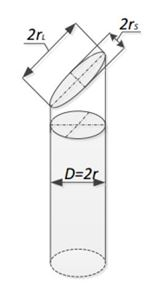
\includegraphics{../images/cut_fiber.JPG} \\ \addlinespace
\bottomrule
\end{longtable}
\end{frame}

\begin{frame}{fiber in spherical coordinates}
\protect\hypertarget{fiber-in-spherical-coordinates}{}
\begin{figure}
\centering
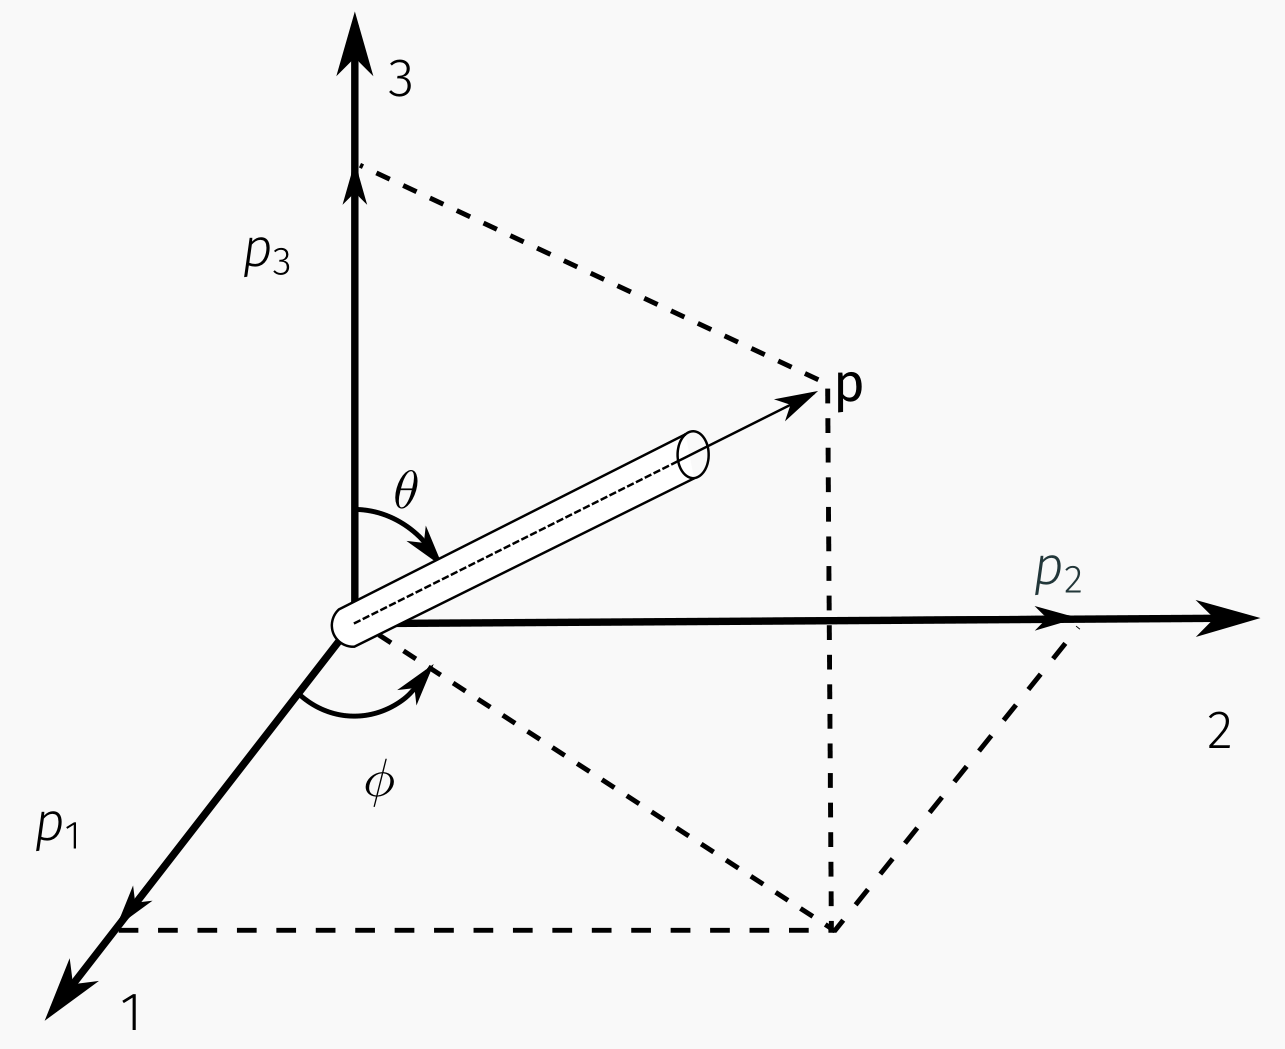
\includegraphics{../images/single_fiber.png}
\caption{Relating the spherical coordinate system to direction vectors
to describe fiber orientation}
\end{figure}

\begin{longtable}[]{@{}
  >{\raggedright\arraybackslash}p{(\columnwidth - 0\tabcolsep) * \real{0.07}}@{}}
\toprule
\endhead
\#\# fiber direction components \\ \addlinespace
\textbar{} Component \textbar{} Definition \textbar{} \textbar{} ---
\textbar{} --- \textbar{} \textbar{} \(p_1\) \textbar{}
\(\sin \theta \cos \phi\) \textbar{} \textbar{} \(p_2\) \textbar{}
\(\sin \theta \sin \phi\) \textbar{} \textbar{} \(p_3\) \textbar{}
\(\cos \theta\) \textbar{} \\ \addlinespace
\bottomrule
\end{longtable}
\end{frame}

\begin{frame}{measurements}
\protect\hypertarget{measurements}{}
\begin{figure}
\centering
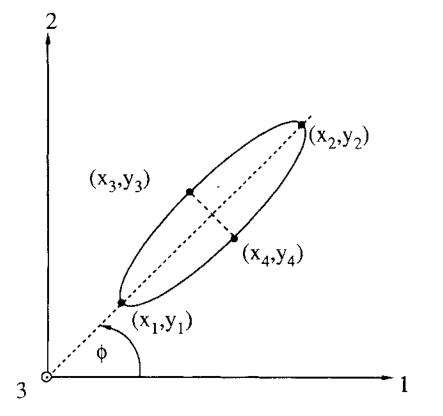
\includegraphics{../images/coordinates.PNG}
\caption{Defining some terms for analyzing the cross-section of an
elliptical fiber cut. Phi is the angle between the major axis of the
ellipse and the 1 axis, x1, y1 mark the bottom left point of the
ellipse, x2, y2 mark the upper right point of the ellipse (the major
axis), while x3,y3 and x4,y4 mark the ends of the minor axis}
\end{figure}

\begin{longtable}[]{@{}
  >{\raggedright\arraybackslash}p{(\columnwidth - 0\tabcolsep) * \real{0.07}}@{}}
\toprule
\endhead
\#\# calculations \\ \addlinespace
- We find the major (\emph{M}) and minor (\emph{m}) axes
using \\ \addlinespace
\(\begin{aligned}
m &= \sqrt{(x_3-x_4)^2+(y_3-y_4)^2}\\
X &= x_1-x_2\\
Y &= y_1-y_2\\
M &= \sqrt{X^2-Y^2}
\end{aligned}\) \\ \addlinespace
\bottomrule
\end{longtable}
\end{frame}

\begin{frame}{orientation tensor}
\protect\hypertarget{orientation-tensor}{}
\begin{itemize}
\tightlist
\item
  We can now calculate angles using
\end{itemize}

\[\sin \phi = \frac{Y}{M} \cos \phi = \frac{X}{M} \cos \theta = \frac{m}{M} \sin \theta = \sqrt{1-\frac{m^2}{M^2}}\]

\begin{longtable}[]{@{}
  >{\raggedright\arraybackslash}p{(\columnwidth - 0\tabcolsep) * \real{0.07}}@{}}
\toprule
\endhead
\#\# microscopy \\ \addlinespace
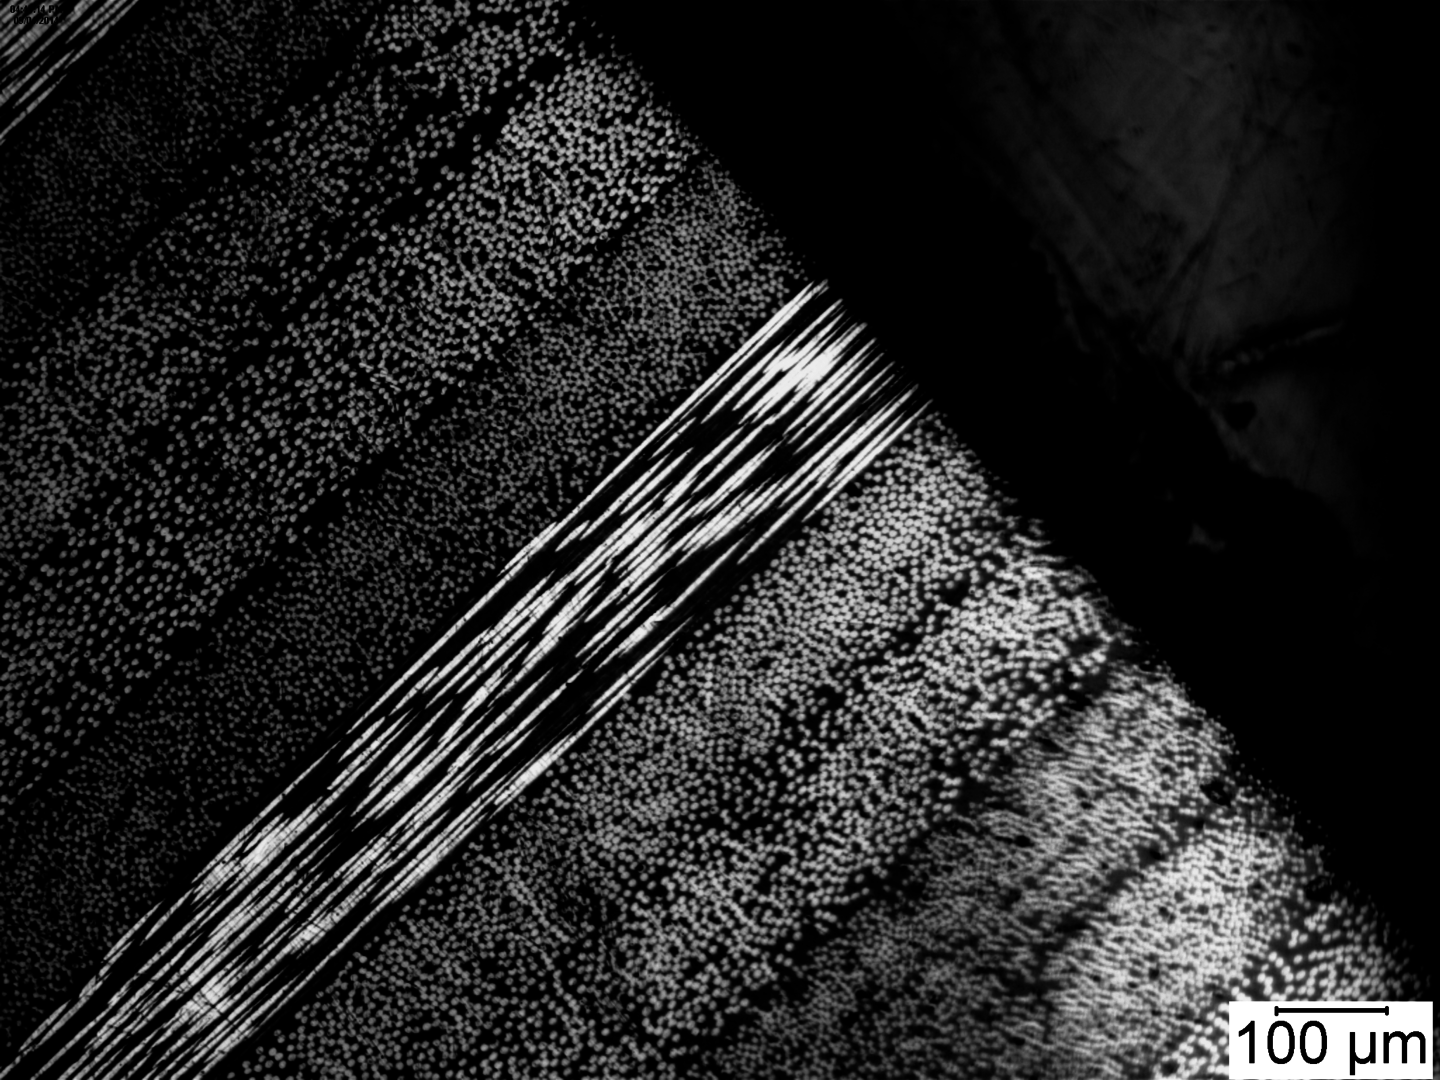
\includegraphics{../images/plies.png} \\ \addlinespace
\bottomrule
\end{longtable}
\end{frame}

\begin{frame}{microscopy}
\protect\hypertarget{microscopy-1}{}
\begin{figure}
\centering
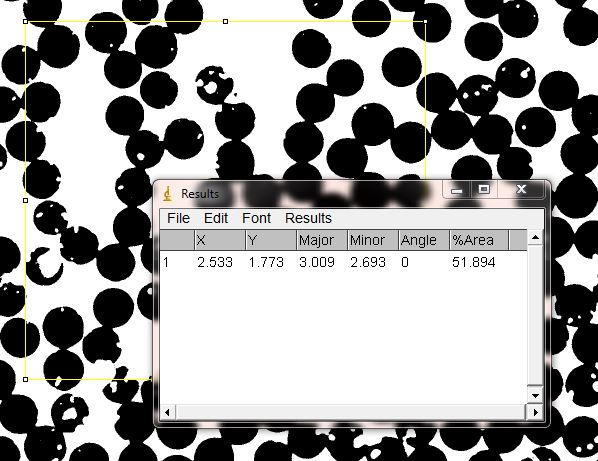
\includegraphics{../images/thresh1.png}
\caption{An image from some analysis to find the volume fraction of
fibers in an image.}
\end{figure}

\begin{longtable}[]{@{}
  >{\raggedright\arraybackslash}p{(\columnwidth - 0\tabcolsep) * \real{0.07}}@{}}
\toprule
\endhead
\#\# microscopy \\ \addlinespace
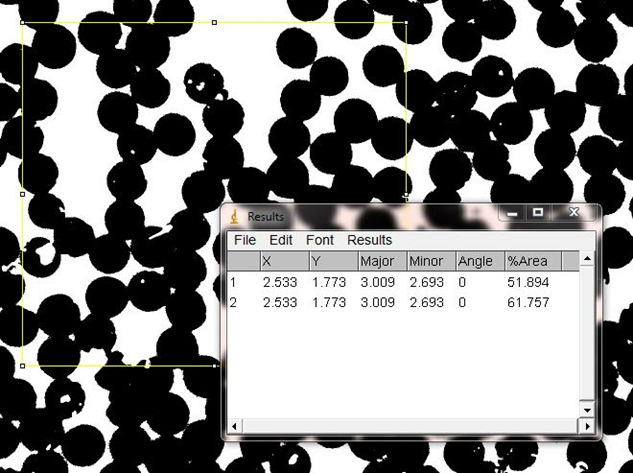
\includegraphics{../images/thresh2.png} \\ \addlinespace
\bottomrule
\end{longtable}
\end{frame}

\begin{frame}{microscopy}
\protect\hypertarget{microscopy-2}{}
\begin{figure}
\centering
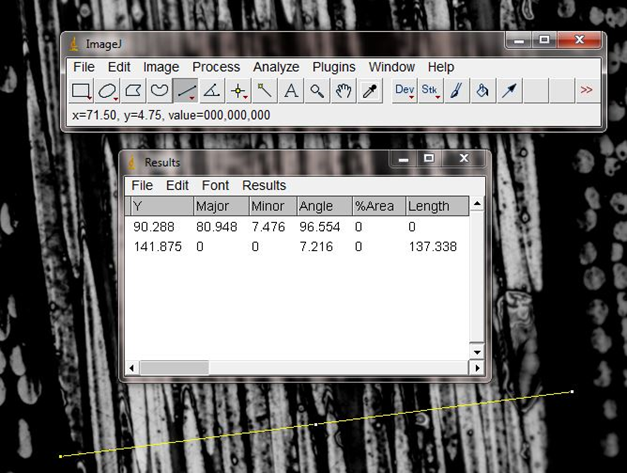
\includegraphics{../images/ply_thickness.png}
\caption{Ply thickness can be measured from a microscopic image}
\end{figure}

\begin{longtable}[]{@{}
  >{\raggedright\arraybackslash}p{(\columnwidth - 0\tabcolsep) * \real{0.07}}@{}}
\toprule
\endhead
\#\# microscopy \\ \addlinespace
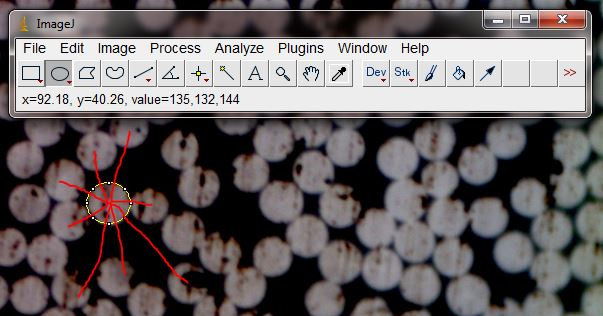
\includegraphics{../images/spacing.png} \\ \addlinespace
\bottomrule
\end{longtable}
\end{frame}

\begin{frame}{software}
\protect\hypertarget{software}{}
\begin{itemize}
\tightlist
\item
  If you have to do a lot of microscopy measurements, contact
  Dr.~Sharma, he wrote an automated measurement tool
\item
  Otherwise you can use
  \href{https://imagej.nih.gov/ij/download.html}{imageJ}
\end{itemize}

\begin{longtable}[]{@{}
  >{\raggedright\arraybackslash}p{(\columnwidth - 0\tabcolsep) * \real{0.07}}@{}}
\toprule
\endhead
\#\# microscopy \\ \addlinespace
- Need to account for bias in measurement (more likely to see fibers
coming out of plane) - There is some ambiguity in fiber angle - Fiber at
(\(\phi, \theta\)) is not distinguishable from (\(\phi + \pi, \theta\))
- In the second-order orientation tensor, this affects \(a_{23}\) and
\(a_{13}\) \\ \addlinespace
\bottomrule
\end{longtable}
\end{frame}

\begin{frame}{serial sectioning}
\protect\hypertarget{serial-sectioning}{}
\begin{itemize}
\tightlist
\item
  Serial sectioning is a method where you continually polish a specimen
  after photographing it
\item
  After photograph you grind and polish, then photograph and repeat
\item
  Gives the full 3D state of orientation, but is difficult
\end{itemize}
\end{frame}

\begin{frame}{CT Scanning}
\protect\hypertarget{ct-scanning}{}
\begin{itemize}
\tightlist
\item
  Even if a CT Scan cannot resolve down to fiber resolution, the
  gradient information can give an idea of fiber orientation
\item
  This method is not very precise
\item
  But it can view the full-field and detect many forms of damage without
  destroying a part
\item
  At the micro-scale full orientation can be obtained, but this is not
  practical for large parts
\end{itemize}
\end{frame}

\end{document}
